\section{Data}
\label{sec:data}

\begin{figure*}[t]
  \centering
  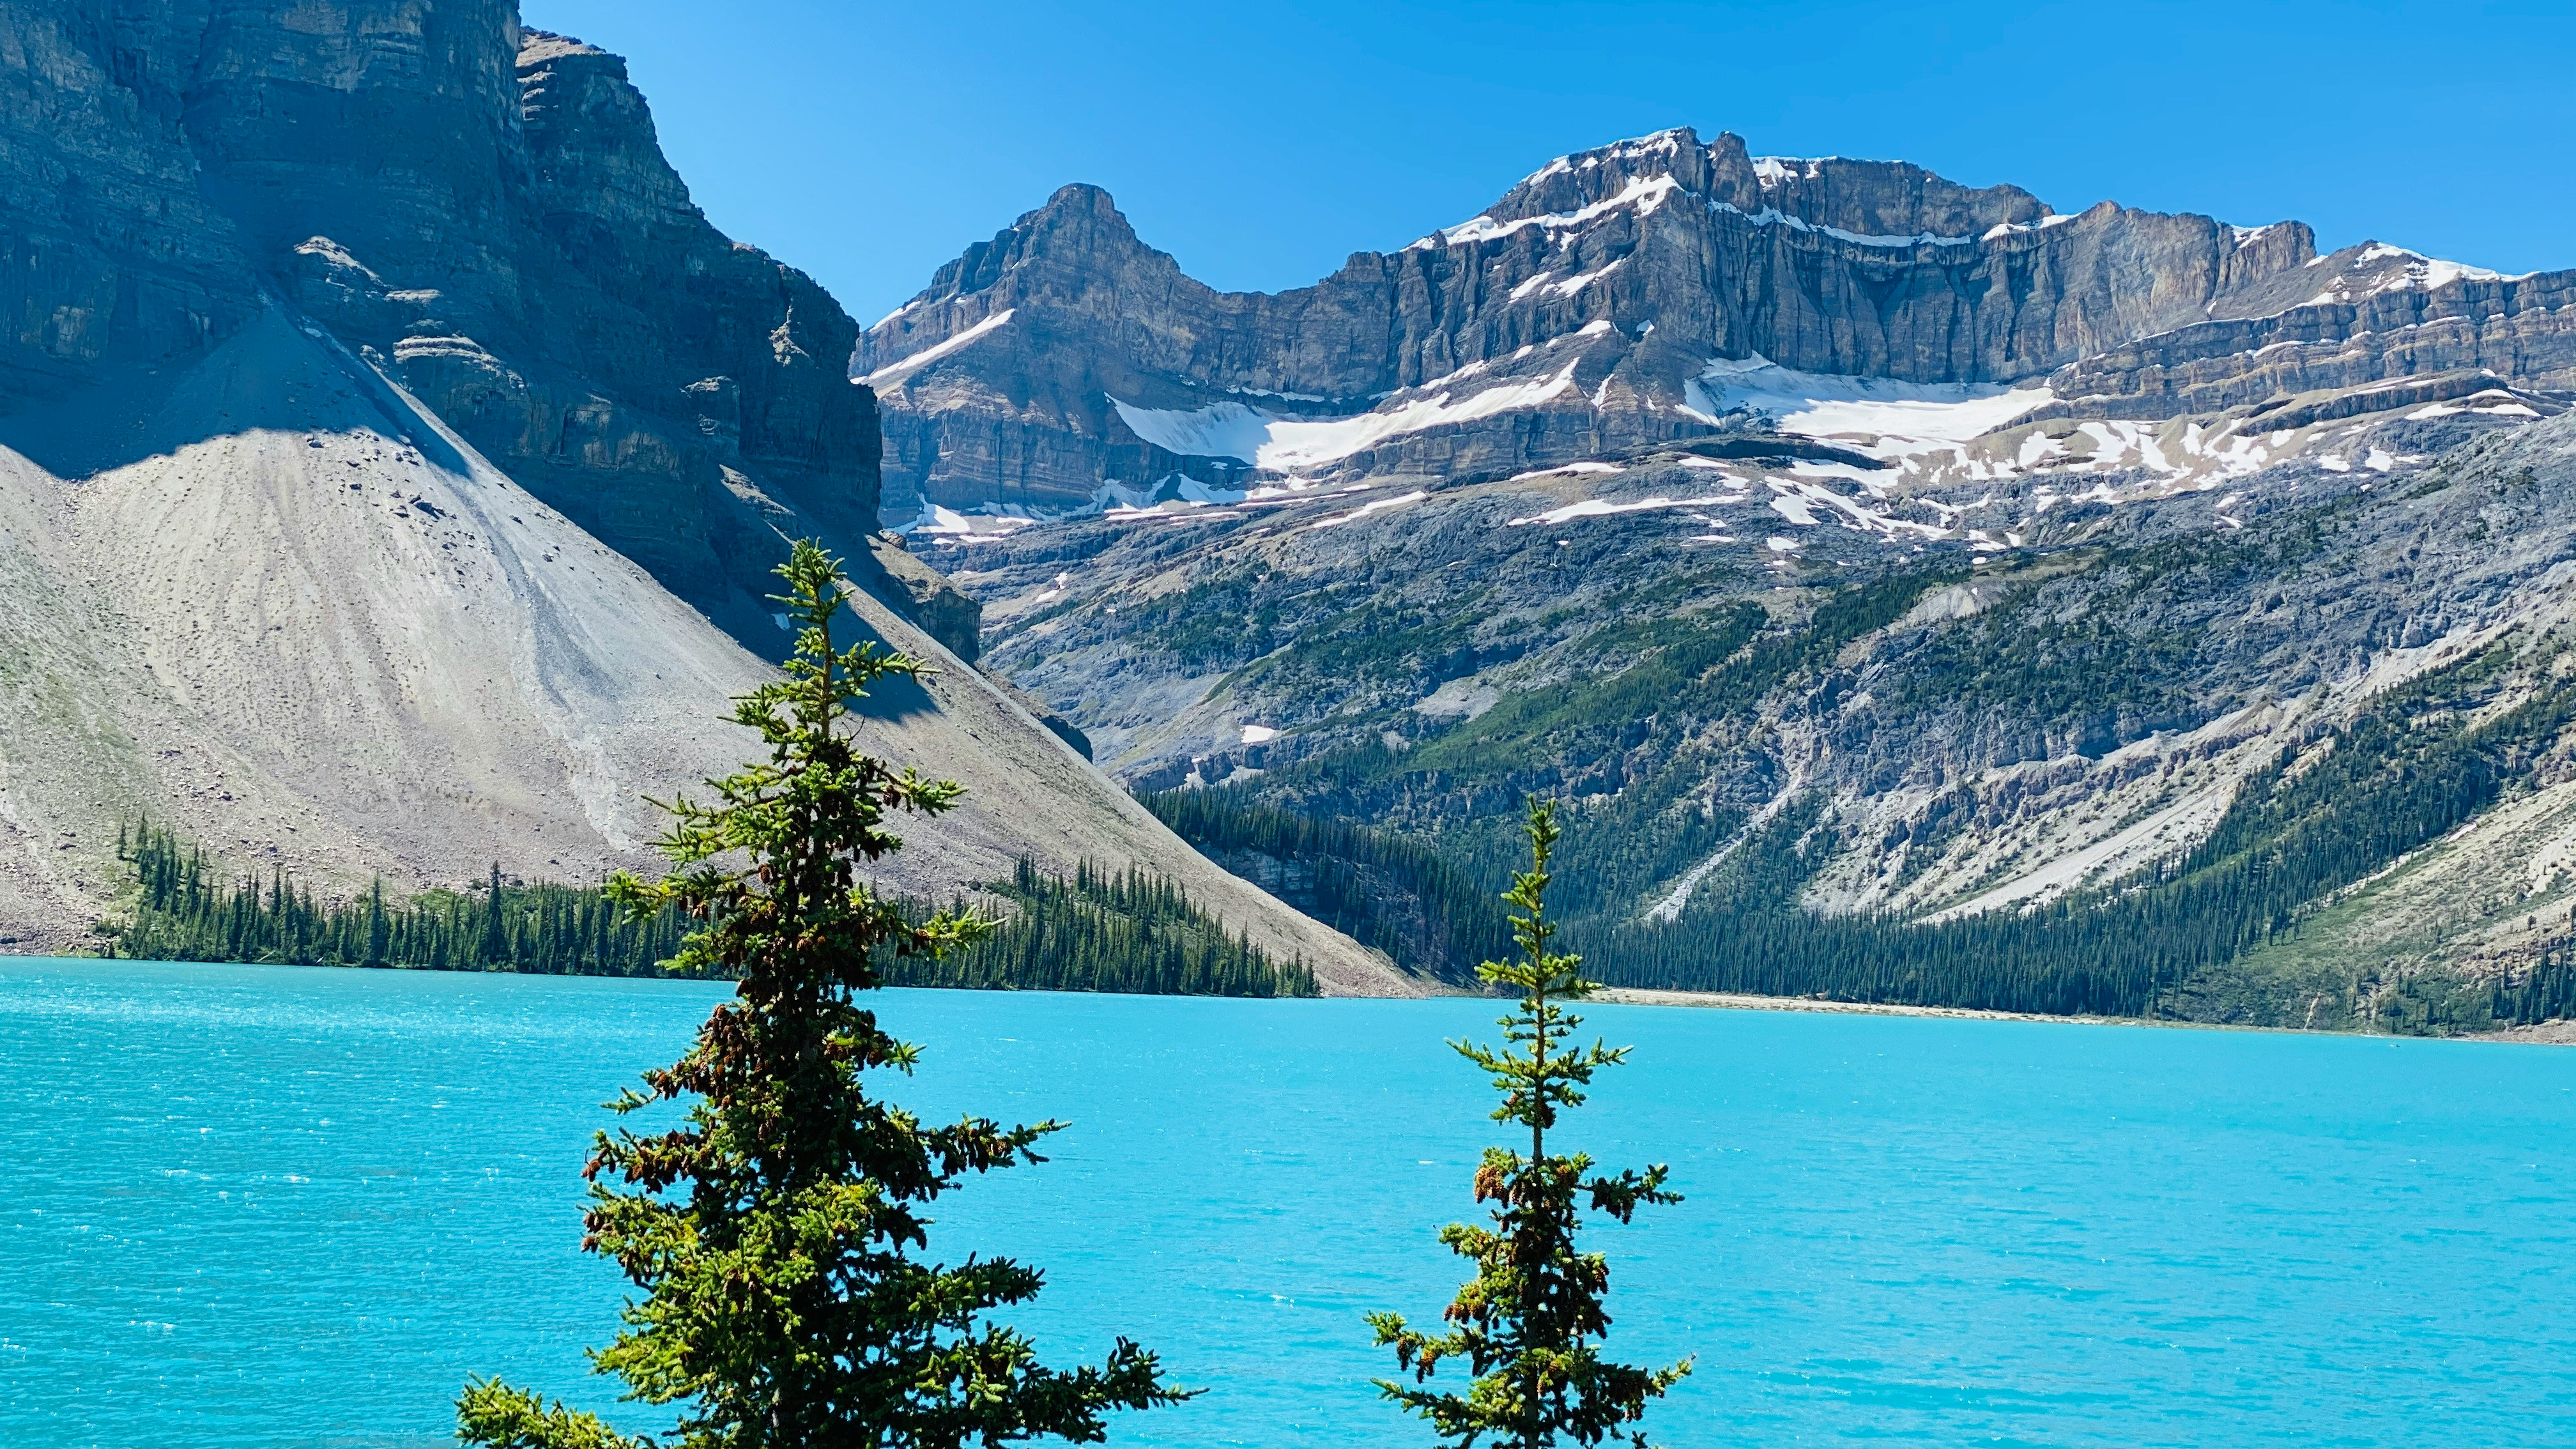
\includegraphics[width=0.92\linewidth]{pngs/image2.png}
  \caption{\textbf{Data pipeline.} Replace this placeholder with a dataset construction, preprocessing, or annotation workflow.}
  \label{fig:data_pipeline}
\end{figure*}

Describe the data sources, collection protocol, filtering criteria, annotation process, and dataset splits.
Include enough detail for readers to understand the scope and limitations of the data without exposing private or unreleased information.

\textbf{Collection.}
Explain where the data comes from and what inclusion criteria were applied.
If applicable, report the number of samples, domains, classes, annotators, or acquisition devices.

\textbf{Preprocessing.}
Describe cleaning, normalization, deduplication, quality control, and format conversion.
Reference Figure~\ref{fig:data_pipeline} if the pipeline is shown visually.

\textbf{Splits and Usage.}
State how training, validation, and test splits are constructed.
Mention measures taken to prevent leakage between splits.

\textbf{Ethics and Licensing.}
Summarize consent, privacy, licensing, and safety considerations when they apply.
For public datasets, cite the original sources, such as a placeholder reference~\cite{sample_reference}.
